\subsection{有効粘度の評価}
Fig.\ref{fig:estimate_eff_viscocity}はせん断速度と有効粘度の関係を表す.

    \begin{figure}[htbp]
        \centering
        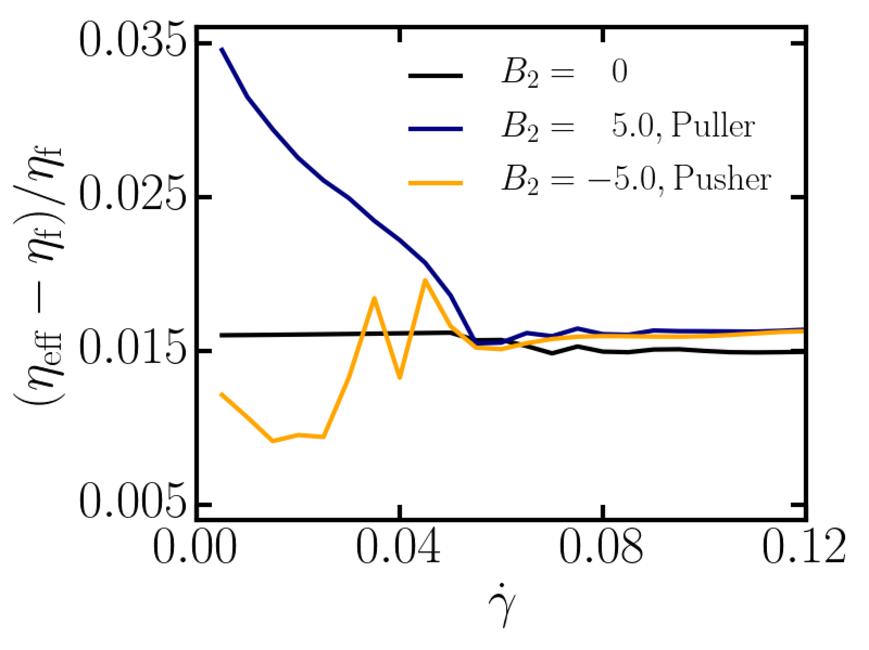
\includegraphics[scale=0.5]{/Users/taiga/Projects/lab/thesis/components/chapter4/figs/gammadot_vs_eff_viscosity.pdf}
        \caption{せん断速度と有効粘度の関係}
        \label{fig:estimate_eff_viscocity}
    \end{figure}

\noindent
このグラフから,せん断速度が小さい領域では,$B_2 > 0$のPuller型は有効粘度を大きくする方向に,
$B_2 < 0$のPusehr型は有効粘度を小さくする方向にはたらいていることが分かる.
また,せん断速度が大きい領域ではsquirmerの種類によらず,ほぼ等しい有効粘度を示していることが分かる.
